\documentclass[border=2pt]{standalone}
\usepackage{tikz}
\usepackage{amsmath,amssymb}
\usetikzlibrary{positioning,arrows.meta,calc}

\begin{document}
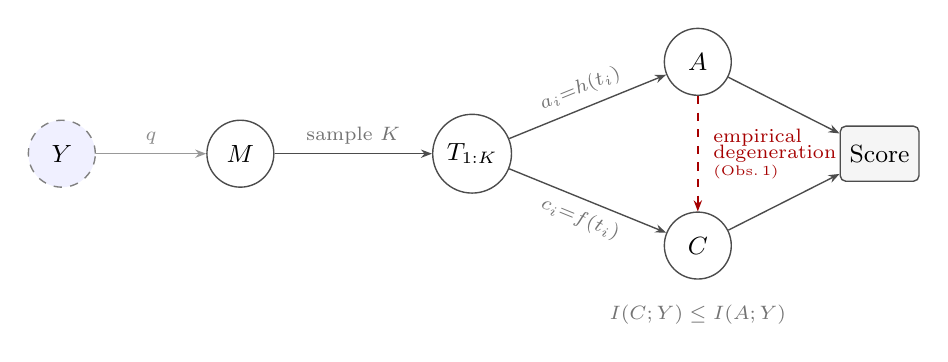
\begin{tikzpicture}[
  every node/.style={font=\small},
  main/.style={circle, draw=black!70, fill=white, minimum size=0.85cm,
               line width=0.5pt, font=\small},
  score/.style={rectangle, draw=black!70, fill=gray!8, rounded corners=2pt,
                minimum height=0.7cm, minimum width=1cm, line width=0.5pt,
                font=\small},
  gt/.style={circle, draw=black!50, fill=blue!6, minimum size=0.85cm,
             line width=0.5pt, font=\small, dashed},
  arr/.style={-{Stealth[length=4pt,width=3pt]}, line width=0.5pt, black!70},
  degen/.style={-{Stealth[length=4pt,width=3pt]}, line width=0.6pt,
                dashed, red!65!black},
  info/.style={font=\scriptsize, text=black!55, align=center},
]

% Horizontal layout: Y  M -> T -> (A,C) -> S
\node[gt] (Y) {$Y$};
\node[main, right=1.4cm of Y] (M) {$M$};
\node[main, right=2cm of M] (T) {$T_{1{:}K}$};
\node[main, above right=0.5cm and 2.2cm of T] (A) {$A$};
\node[main, below right=0.5cm and 2.2cm of T] (C) {$C$};
\node[score, right=1.8cm of $(A)!0.5!(C)$] (S) {Score};

% Solid arrows
\draw[arr, black!40] (Y) -- (M) node[midway, above, font=\scriptsize, text=black!45] {$q$};
\draw[arr] (M) -- (T) node[midway, above, font=\scriptsize, text=black!55] {sample $K$};
\draw[arr] (T) -- (A) node[midway, above, sloped, font=\scriptsize, text=black!55] {$a_i{=}h(t_i)$};
\draw[arr] (T) -- (C) node[midway, below, sloped, font=\scriptsize, text=black!55] {$c_i{=}f(t_i)$};
\draw[arr] (A) -- (S);
\draw[arr] (C) -- (S);

% Dashed degeneration edge A -> C
\draw[degen] (A) -- (C)
  node[midway, right=2pt, font=\scriptsize, text=red!65!black, align=left]
  {empirical\\[-2pt]degeneration\\[-2pt]{\tiny(Obs.\,1)}};

% DPI annotation
\node[info, below=0.2cm of C] {$I(C;Y) \leq I(A;Y)$};

\end{tikzpicture}
\end{document}
